\documentclass[../dissertation.tex]{subfiles}

\begin{document}

\section{ROS (Robot Operating System)}
\label{background-ros}

The specific focal point of this investigation is ROS (Robot Operating System). ROS is one of the most popular robotic middlewares, with a large active community of users, and ongoing development. However, much of the existing knowledge about ROS' communication performance is anecdotal and scattered across posts on websites such as StackOverflow or individual blogs.

ROS's primary goal is one of sharing and collaboration. Robotic systems often use custom-created software such as driver software and higher-level algorithms like pathing. ROS creators want to make this custom created software reusable across a wide variety of platforms, reducing the amount of repeated independent development, and allowing for faster creation of useful robots. On top of this primary goal, ROS also aims to be very thin, allow libraries to be ROS-agnostic, be language independent, allow easy testing (unit and integration), and easily scale to large systems. ROS has two implementations: `roscpp' using C++, and `rospy' using Python. These two implementations generally mimic each other in as many ways as possible, however sometimes the behaviours of these implementations differ due to language differences.

ROS achieves it's primary goal via the use of packages. A ROS package contains all the information and files needed to perform one task. This can include code, datasets, and configuration files. ROS's computation and communication units are nodes. A ROS node represents a process that performs a particular computation. A package generally contains one or more nodes. Nodes can communicate between each other directly with the use of messages, or invoke services. The ROS Master node is a particular node which must run on every ROS system. The Master provides look-up services for nodes (so that they can find each other) with a URL-like system. The Master also provides the Parameter Server. The parameter server allows for nodes to store and retrieve data at run-time from a centralised, shared dictionary.

The majority of inter-node communication is achieved using topics. A topic represents a strongly typed message bus to which one or more nodes publish messages, and zero or more nodes subscribe to receive published messages. There are no access permissions to a topic, any node can publish or subscribe as long as they use the correct data type. Publishing to a ROS topic involves the following steps:

\begin{enumerate}
  \item A message object is constructed containing the data to be sent
  \item The message is placed in a queue of messages to be sent from that node
  \item A message is pulled off the queue, and serialized
  \item The serialized message is written in to a buffer
  \item The buffer is written to the transport of every current subscriber
\end{enumerate}

On the subscriber's end, the following occurs:

\begin{enumerate}
  \item An incoming stream is written to an internal buffer
  \item The buffer is split in to serialized messages
  \item A message is deserialized to an object, and placed in to the subscriber's queue
  \item The subscriber pulls message objects off the queue
\end{enumerate}

\begin{figure}[H]
\centering
\includegraphics[width=0.5\textwidth]{images/background/ROS_Queues.png}
\caption{ROS process of sending a message from Node 1 to Node 2. Note that the internal buffers are omitted from this figure.}
\end{figure}

Another option for inter-node communication is to use services. A service represents a restricted version of publisher/subscriber which implements a request/response interaction. When a node invokes a service, it sends a request (a message of a specific type) to the node implementing the service, and waits for the response. The response is sent back as another type (although possibly the same type).

The ROS community highly favours open source and sharing, as it aligns with the primary goal of ROS.

\section{Configuration of Robots}
\label{background-robot-config}

This project involved the use of 9 identical robot cars with front-wheel steering. The cars were previously built from a Sunfounder Smart Video Car Kit for Raspberry Pi\cite{SunfounderRobotCarKit}.

The car kit includes the physical pieces required to construct a robot car, such as a frame, gears, wheels, motors, step-down converters, and wires. The kit also includes a USB camera, and Wi-Fi adapter. It also includes a space for a Raspberry Pi (B+/2/3) to be seated. The robot cars were fitted with one Raspberry Pi 3 Model B each.

\begin{figure}[H]
\centering
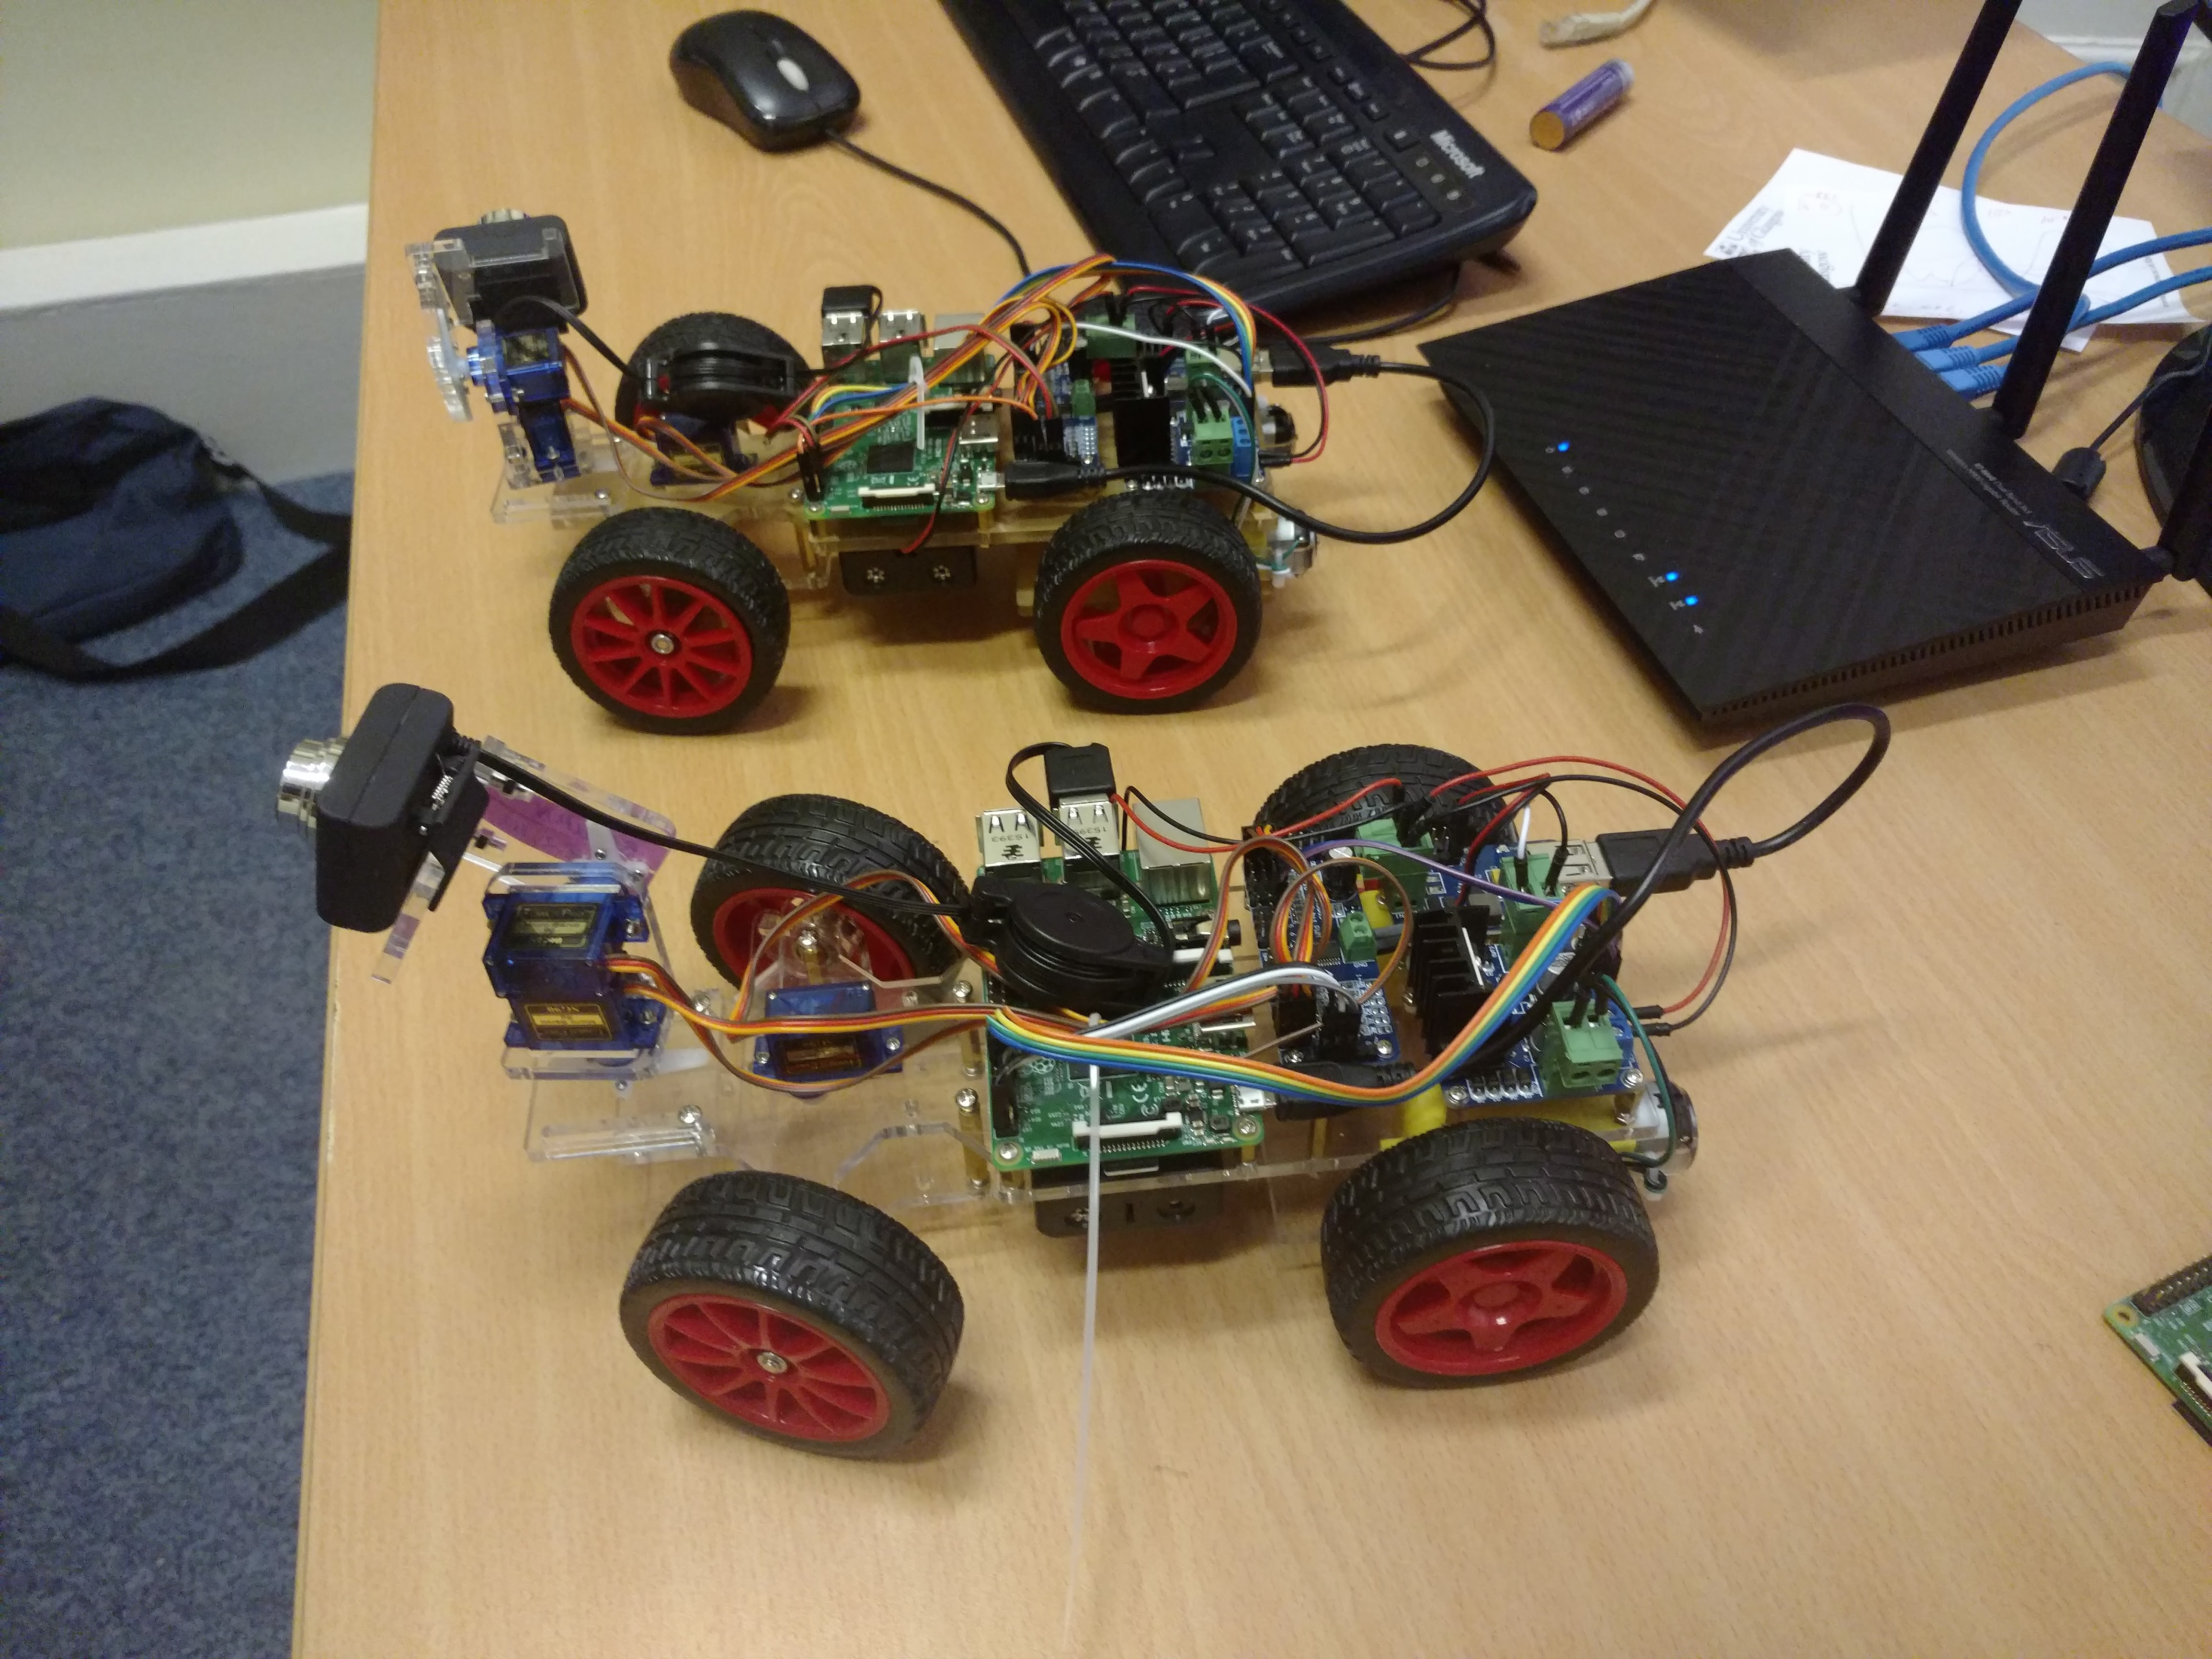
\includegraphics[width=0.7\textwidth]{images/background/robot-cars.jpg}
\caption{Photo of 2 of the Sunfounder Robot Cars}
\end{figure}

\end{document}
